% Created 2010-08-11 Wed 16:22
\documentclass[11pt,a4paper,oneside,draft]{book}
\usepackage[utf8]{inputenc}
\usepackage[T1]{fontenc}
\usepackage[draft=false]{hyperref}
\usepackage[english,nynorsk]{babel} % or whatever language
\usepackage{apacite} % after babel
\usepackage{natbib}
\usepackage{graphics}
\usepackage[author=]{fixme}
\fxusetheme{colorsig}

\usepackage{amsmath} % for \operatorname

\usepackage{linguex} 

\usepackage{pslatex}
% \usepackage{pdfsync} % bug with glosses ( \exg. in linguex )

\usepackage{tikz-qtree}
\usepackage{avm}
\avmfont{\sc}
\avmoptions{sorted,active}
\avmvalfont{\rm}
\avmsortfont{\scriptsize\it}
\usepackage{algorithm2e}
\SetAlgorithmName{Funksjon}{fn}{liste over psevdokode}
%\SetAlgoFuncName{Funksjon}{} % for some reason gets no numbering TODO

\newcommand{\xbar}{$\rm\overline{X}$}
\newcommand{\F}[2]{\textsc{#1}\ensuremath{_{#2}}}
\newcommand{\OBLben}{\F{obl}{ben}}
\newcommand{\OBJben}{\F{obj}{ben}}
\newcommand{\OBJ}{\F{obj}{}}
\newcommand{\OBJs}{\F{obj~}{}}
\newcommand{\ADJ}{\F{adj}{}}
\newcommand{\ADJs}{\F{adj~}{}}
\newcommand{\XCOMP}{\F{xcomp}{}}
\newcommand{\XCOMPs}{\F{xcomp~}{}}
\newcommand{\SUBJ}{\F{subj}{}}
\newcommand{\SUBJs}{\F{subj~}{}}
\newcommand{\PRED}{\F{pred}{}}
\newcommand{\falign}{\ensuremath{\operatorname{\emph{falign}}}}
\newcommand{\fpairs}{\ensuremath{\operatorname{\emph{fpairs}}}}
\newcommand{\Bleu}{\textsc{Bleu}}

\title{Syntaktisk informert frasesamanstilling }
\author{Kevin Brubeck Unhammer}
\date{11/08, 2010}

\begin{document}

\maketitle

\setcounter{tocdepth}{4}
\tableofcontents
\vspace*{1cm}

\listoffixmes

\chapter{Innleiing}
\label{sec-1}

\label{SEC:innleiing}

\fxnote{TODO: abstract/samandrag}

Denne masteroppgåva utforskar kva det vil seie at to uttrykk er
omsetjingar av kvarandre, og korleis me automatisk kan generere og
evaluere samanstilling (\emph{alignment}) av uttrykk som
står i eit slikt omsetjingsforhold. 

Omsetjingsforhold finn me mellom setningar i kontekst på ulike språk,
men me kan au finne ulike typar ekvivalensforhold (samanstillingar)
mellom frasar innanfor setningane, og mellom lingvistiske
skildringar av setningane. I samanheng med XPar-prosjektet
\citep{xpar2008rcn} har eg sett på metodar for automatisk
frasesamanstilling – å finne omsetjingsforhold mellom grupper av
fleire ord. Resultatet blir ein \emph{annotasjon}, endå ei lingvistisk
skildring av tekstene.



Det at me kan omsetje mellom lingvistiske skildringar
(t.d. trekkstrukturane til dei grammatiske rammeverka HPSG eller LFG)
gjer det tydeleg at me arbeider med ein \emph{modell} av språket; ulike
skildringar kan vere sanne innanfor modellen, utan at modellen er lik
språket. Sjølve omsetjingsforholdet er au ein teoretisk storleik, og
me kan leggje ulike kriterium til grunn for å kalle to uttrykk
omsetjingar av kvarandre.

Kriteria avheng av formålet. Samanstillingsannotasjon kan t.d. nyttast
som grunnlag for statistisk eller eksempelbasert maskinomsetjing, i
tillegg til oppbygging av parallelle korpora for meir teoretiske
språkstudie.  For statistisk maskinomsetjing vil alle uttrykk vere
omsetjingar av kvarandre med eit visst sannsyn (kanskje null), ein
har vanlegvis ikkje kriterium som krev lingvistisk analyse. Når
samanstillinga skal nyttast i parallelle korpora for lingvistiske
undersøkingar vil ein kanskje ha krav om at uttrykk som skal lenkjast
er «like» på eit eller anna mål, utover at dei har opptredt saman
ofte; i den manuelle samanstillinga i \citet{samuelsson2006pap} har
dei t.d. ein del reint semantiske kriterium for å opprette
fraselenkjer i ein parallell trebank, men dei har ikkje krav om
syntaktisk likskap.

Xpar-prosjektet, som denne masteroppgåva er ein del av, har mellom
anna som mål å oppdage relasjonar mellom grammatiske funksjonar,
tematiske roller og kasusmarkering, ved hjelp av parallelle trebankar
annotert med djupe grammatiske analysar.  Samanstillinga planlagt der
krev i større grad syntaktisk likskap for å kalle to uttrykk
omsetjingar, men kan difor au tene på det at dei grammatiske analysane
er utvikla med tanke på å vere så parallelle som mogleg.  Dei
grammatiske analysane er gjort i leksikalsk-funksjonell grammatikk,
LFG \citep{bresnan2001lfs}. Ei grammatisk analyse i LFG involverer
både konstituentstruktur (c-struktur) og funksjonell struktur
(f-struktur). Konstituentstrukturen liknar på frasestrukturtrea frå
andre grammatiske tradisjonar. Dei funksjonelle strukturane er
trekkstrukturar, som mellom anna representerer avhengnadsforhold
mellom syntaktiske funksjonar som predikat, subjekt og objekt, i
tillegg til å halde informasjon om grammatiske trekk som genus, tal
eller kasus. Nodar i c-strukturen kan spesifisere informasjon på ulike
stader i f-strukturen\footnote{Ved c-struktur-f-strukturavbildinga $\phi$, ein funksjon som
        tek ein c-strukturnode og returnerer ein (delvis) f-struktur. }.

I XPar-prosjektet vil ein finne ut om metodar for frasesamanstilling
kan tene på det at LFG-grammatikkane for dei ulike språka er skrivne
med same prinsipp lagt til grunn; to parallellstilte setningar bør ha
f-strukturar som er like nok til at me kan samanstille frasar ved
hjelp av likskapen mellom f-strukturane. I \citet[s.~72]{dyvik2009lmp}
finn me følgjande hypotese:

\begin{quote}
On the basis of monolingual treebanks constructed from a parallel
corpus by means of parallel grammars it will be possible to achieve
automatic word and phrase alignment with significantly higher
precision and recall than hitherto achieved through other means.
\end{quote}

kor «parallel grammars» her krev parallellisme i både f-struktur og
c-struktur.

Men i tillegg til at ein kanskje kan få betre skåre på desse
kvantitative måla, vil lenkjer mellom f-strukturar gi informasjon som
er kvalitativt forskjellig frå det ein kan få med å berre sjå på
lenkjer mellom ord, N-gram eller konstituentar.

I denne masteroppgåva spesifiserer eg kva for lenkjer mellom
f-strukturar og c-strukturnodar me ønskjer, implementerer eit program
\texttt{lfgalign} som automatisk finn samanstillingar med slike lenkjer,
evaluerer resultatet av å køyre programmet mitt, og samanliknar dette
med kva me kan få frå andre metodar.

Programmet \texttt{lfgalign} opprettar frasesamanstillingar med hjelp av
f-strukturinformasjonen gitt av dei parallelle grammatikkane, og
bottom-up-informasjon om kva for ordsamanstillingar som er
moglege. F-strukturane avgrensar igjen kva for ordsamanstillingar som
er moglege, og kva for c-strukturnodar (syntaktiske frasar) som kan
lenkjast.


\section{Vegkart}
\label{sec-1.1}

I neste kapittel ser eg på andre metodar for frasesamanstilling.

I kapittel \ref{SEC:ideell} går eg gjennom kva me ønskjer av ei
frasesamanstilling når formålet m.a. er å oppdage relasjonane mellom
syntaktiske funksjonar, kasusmarkering og tematiske roller med hjelp
av ein parallell trebank. Dette ender opp i ei liste med «krav» som
samanstillingane må fylle for å vere lovlege, og som implementasjonen
av den automatiske frasesamanstillinga (kapittel
\ref{SEC:implementasjon}) må følgje.

Eg evaluerer samanstillingane som kjem ut av denne metoden i kapittel
\ref{SEC:diskusjon}, og samanliknar dei med det som er mogleg der me
berre har konstituentstruktur (syntaktiske tre) i tillegg til
ordsamanstilling.

Eg nyttar språka georgisk og norsk i evalueringa, hovudsakleg fordi
dei er svært ulike syntaktisk og morfologisk; Georgisk er mellom anna
eit pro-drop-språk, med friare ordfølgje og rikare morfologi enn
norsk.  \fxnote{fortelje om georgisk i kap.5 heller}

Sidan eg ikkje har tilgang på ferdig setningssamanstilt georgisk-norsk
parallelltekst, blir det vanskeleg å køyre den statistiske
ordsamanstillinga som er vanleg som første steg i N-grambaserte
metodar (utan ein god del forarbeid). Difor konsentrerer eg meg i
evalueringa om eit testkorpus kor eg manuelt gjer
ordsamanstillinga. Eg veit heller ikkje enno om nokon statistisk
parsar av høg kvalitet for georgisk, men testkorpuset er ferdig parsa
med LFG-parsaren frå \citet{meurer2008cgg}, c-strukturnodane avgrenser
då kva som er ein syntaktisk konstituent.


\chapter{Bakgrunn og omgrepsavklaring}
\label{sec-2}

  \label{SEC:bakgrunn}
\fxnote{TODO (innleiing?):\\
   - reine N-gram-samanstillingar, dependensbaserte\\
   - ulike formål for samanstilling gir ulike metodar\\
   - kort oversyn over LFG-termar \\
}
\section{\textbf{SKRIV} Relaterte metodar}
\label{sec-2.1}

Automatisk frasesamanstilling er eit nytt felt. Det finst allereie
veldig gode system for automatisk setningssamanstilling, og automatisk
samanstilling av ord har komme langt, men nivåa mellom ord og setning
ser ut til å by på fleire problem. \fxnote[inline,nomargin]{«by på
fleire problem» -- weasel wording, TODO omskriv.} Dei ulike tilnærmingane
som finst er prega av formåla til utviklarane. Det er verdt å merkje
seg at ordet «frase» ofte blir nytta i litteraturen om strenger av ord
(N-gram) som ikkje treng vere syntaktiske konstituentar, igjen
avhengig av formålet med metoden.

Innanfor korpuslingvistikken har t.d. \citet{piao2001mwu} nytta enkel
kollokasjonsinformasjon for å først finne sannsynlege nominale frasar
på engelsk og kinesisk (dvs. «chunking»), og så samanstille desse; her
er evalueringsgrunnlaget rett og slett ein manuell gjennomgang av dei
mest sannsynlege omsetjingane dei får. \fxnote{fleire slike? meir om
dette, algoritmen}

Den manuelle frasesamanstillinga i \citet{samuelsson2006pap}, nemnt
over, blei nytta som evalueringsstandard for den automatiske metoden i
\citet{samuelsson2007apa}.  Her kjem frasesamanstillinga frå ei
ordsamanstilling, der berre N-gram som svarer til ein syntaktisk node
blir lenkja som frasar (meir om denne metoden nedanfor). Formålet er å
lage ein parallell trebank, kor det altså er unyttig å lenkje «frasar»
som \emph{ikkje} er konstituentar.

Sjølv om fraselenkjer kan vere nyttige i korpuslingvistikken er det
hovudsakleg innanfor statistisk maskinomsetjing at ein har forska på
samanstilling av frasar. \citet{koehn2003spb} gir ei grundig
evaluering av ulike statistiske metodar for frasesamanstilling til
bruk i stokastisk maskinomsetjing. Dei nyttar \Bleu-skåren til å
rangere resultata
\citep[Papineni~et~al.,~2001,~i][s.~51]{koehn2003spb}, som gir ei
rangering ved (N-grambasert) samanlikning med ferdig omsett tekst.

Den første metoden, \emph{AP}, er reint N-grambasert. Dei nyttar verktøyet
Giza++ \citep[Och~og~Ney,~2000,~i][s.~50]{koehn2003spb} til å indusere
ordsamanstilling frå eit setningssamanstilt korpus (vha. «modell 4»
for ordsamanstilling, utvikla ved IBM av \citet{brown1993msm}). Denne
samanstillinga er 1-til-n (t.d. eitt engelsk ord til to franske), så
dei finn ordsamanstilling for begge retningar og tek så snittet av alle
moglege N-gramsamanstillingar som ikkje er i konflikt med
ordsamanstillingane. Dei føyer så på ord frå unionen av desse
vha. nokre enkle heuristikkar.

Den andre metoden, \emph{Syn}, tek berre med dei frasane som står under
syntaktiske nodar i eit parsa korpus; frasesamanstillinga til \emph{Syn} er
ein delmengd av den i \emph{AP}. Denne syntaktisk informerte modellen gav
ein mykje dårlegare \Bleu-skåre enn den reint N-grambaserte modellen
(faktisk dårlegare enn omsetjingane frå den opphavlege modell 4 for
ordsamanstilling, utan frasesamanstilling). Dei forklarer dette med
den store mengda uttrykk som ikkje utgjer syntaktiske konstituentar i
følgje parsaren deira, men likevel konsekvent blir omsett til visse
uttrykk på det andre språket (t.d. «es gibt» på tysk til «there is» på
engelsk).

Seinare resultat har vist at ein \emph{kombinasjon} av syntaktisk
informerte metodar med reint N-grambaserte modellar (dvs. i motsetning
til å berre fjerne samanstillingar mellom ikkje-konstituentar) kan
auke skåren i ein maskinomsetjingsevaluering, både om ein som i
\emph{Syn}-modellen nyttar frasestrukturinformasjon, men i endå større
grad om ein nyttar dependendsinformasjon
\citep{tinsley2007ept,hearne2008ccd}. Dette er interessant med tanke
på at LFG-analysane gir begge typar informasjon.

\citet{riezler2006gmt} utvikla ein metode for å kombinere frasebasert
statistisk maskinomsetjing med LFG-basert setningsgenerering. Dei finn
ei n-til-m-ordsamanstilling med Giza++ som i metodane over, men parsar
i tillegg setningane i LFG. Dei to moglege f-strukturane som liknar
mest blir valt ut, og frå ordsamanstillinga finn dei
mange-til-mange-korrespondansar mellom substrukturane i
f-strukturane. Ved å leggje til LFG-basert generering fekk det
kombinerte systemet betre resultat på langdistanseavhengnader og
generalisering til nye uttrykk med strukturell likskap til tidlegare
observerte uttrykk.
\fxnote{Dette er motsett retning av det mitt program gjer, nemne
seinare?}

Så langt har eg ikkje komme over metodar som går i motsett retning,
altså prøver å finne eller betre på frase- og ordsamanstilling ut frå
ein LFG-parse -- det er dette som er strategien til programmet
\texttt{lfgalign} i kapittel \ref{SEC:implementasjon} -- men det er stor
overlapp mellom krava som kjem i kapittel \ref{SEC:ideell} og dei gitt
i den første publiseringa i XPar-prosjektet, \citet{dyvik2009lmp}.


\section{\textbf{SKRIV} Eit kort oversyn over leksikalsk-funksjonell grammatikk og terminologi}
\label{sec-2.2}

\label{SEC:omgrepsavklaring}

I dei følgjande kapitla nyttar eg ein del LFG-terminologi (i tillegg
til eit par eigne termar). Difor gir eg her eit kort oversyn over det
som kan vere nytt for dei som er meir vand med andre grammatiske
rammeverk.

\begin{description}
\item [modellteoretisk (vs derivasjonelt)] LFG er eit modellteoretisk,
  ikkje-derivasjonelt, rammeverk for grammatikk.
  \citet{pullum2001dbm} gir ein god gjennomgang av forskjellen mellom
  derivasjonelle (enumerative) grammatikkar og modellteoretiske
  grammatikkar, kor førstnemnde definerer \emph{mengder av uttrykk} ved
  avleiing frå startsymbol, medan sistnemnde gir skildringar av
  \emph{enkeltuttrykk}. Ein modellteoretisk grammatikk kan i tillegg
  skildre strukturen (eller dei moglege strukturane) til \emph{fragment} av
  setningar, og denne strukturen er lik det bidraget som fragmentet
  tilfører skildringa av heile setninga. Det tilsvarande er ikkje
  mogleg å gjere derivasjonelt. \citet[s.~32--33]{pullum2001dbm} gir
  t.d. eit fragment som kjem midt i eit høgreforgreina tre; ein
  derivasjonell skildring ville måtte skildre treet over eller under,
  men utan informasjon om kva som kjem til høgre eller venstre kan me
  ikkje (på ein ikkje-vilkårleg måte) skildre subtreet utanfor
  fragmentet heilt fram til terminal- eller startsymbol.
\item [f-struktur] \ldots{}
\item [c-struktur] \ldots{}
\item [endosentrisitetsprinsippa] \ldots{}
\item [\xbar] \ldots{}
\item [diskontinuerlege konstituentar] \ldots{}
\item [$\phi$] c-struktur-f-strukturavbildinga $\phi$ \ldots{}
\item [$\phi^{-1}$] Det funksjonelle domenet til ein f-struktur er gitt
  ved $\phi^{-1}$, inversen av c-til-f-strukturavbildinga, og
  tilsvarer dei nodane i c-strukturen som projiserer denne
  f-strukturen, t.d. ein VP-node med dominerande IP og CP
  \citep[s.~126]{bresnan2001lfs}. Sidan dette er inversen av ein
  funksjon, kan me ha diskontinuerlege konstituentar i same
  funksjonelle domene (på same måte som ulike argument til ein
  funksjon kan gi same verdi).
\item [fraselenkjer vs frasesamanstilling] Eg nyttar her termane
  \emph{lenkjing} og \emph{samanstilling} i omtrent same tyding som dei engelske
  termane \emph{link} og \emph{alignment}, kor ei samanstilling er ei mengd
  lenkjer. Dette er ekvivalensforhold som me kan finne mellom
  lingvistiske \emph{representasjonar} (f-struktur, c-struktur) eller
  \emph{uttrykk} (ord, setningar); lenkjing mellom dei siste altså er meir
  ateoretisk / datanært.
\end{description}
\chapter{Krav til frasesamanstilling}
\label{sec-3}

\label{SEC:ideell}

\section{Innleiing}
\label{sec-3.1}

I denne delen prøver eg å finne fram til kva som er den best moglege
frasesamanstillinga. Eg argumenterer for at «best» her må tolkast i
forhold til eit formål, her å finne samsvar mellom kasusmarkering og
semantisk rolletildeling. Som utgangspunkt har eg visse krav for
ordsamanstilling gitt i \citet{thunes2003eal}, saman med krava for
frasesamanstilling i \citet{dyvik2009lmp}. Eg viser kvifor ein, for
våre formål, må revidere kravet til Thunes om likskap i
argumentstruktur. Eg gir nokre døme for å grunngje krava i
\citet{dyvik2009lmp}, i tillegg til å utdjupe dei for å gjere dei
enklare å implementere i kapittel \ref{SEC:implementasjon}. Dette
involverer au å omformulere krava for c-struktursamanstilling slik at
dei ikkje refererer til ordlenkjer, berre f-strukturlenkjer. Sidan eit
av måla med Xpar-prosjektet er å finne ut kor mykje
frasesamanstillingsinformasjon me kan få ut av parallellismen i
f-strukturane (eller, sett frå den andre sida, kor uavhengig ein kan
gjere seg av den bottom-up-informasjonen ei ordlenkje gir), blir det
eit avleidd mål å formulere frasesamanstillingskrava med referanse til
f-strukturane der det går an.

\section{Formål med frasesamanstilling}
\label{sec-3.2}

\label{SEC:formaal}

Ei frasesamanstilling er ein slag annotasjon av eit korpus. På same
måte som oppbygginga av eit korpus avheng av formålet til korpuset,
kan ein ikkje definere den ideelle annotasjonen av eit korpus utan å
ta høgd for kva ein skal nytte annotasjonen til.

Me kan illustrere dette med eit enkelt, praktisk døme: ved automatisk
ordklassetagging må ein gjerne avvege mellom dekning (å finne flest
moglege analysar for flest mogleg ord) og presisjon (å berre ende opp
med korrekte analysar).  Viss formålet er å annotere ein
leksikografisk ressurs, vil det vere viktigare med høg dekning på
bekostning av presisjon, sidan leksikografen gjerne leiter etter
nye/kreative bruksområde av ord. Skal taggaren nyttast til
maskinomsetjing i staden, kan ein ikkje nytte meir enn éin analyse til
slutt, så her er presisjon viktigast.

Sjølvsagt kan ein her seie at den \emph{ideelle} annotasjonen vil vere å
berre ha korrekte analysar, men sjølv ved ideelle krav er formålet
viktig: er ein ute etter å finne N-gram som ofte blir omsett med
kvarande, men som \emph{ikkje} er syntaktiske konstituentar, er det klart
at retningslinjene nedanfor ikkje er så nyttige.

Sidan utviklinga av automatisk frasesamanstilling hovudsakleg har
skjedd innanfor frasebasert statistisk maskinomsetjing (PBSMT), kjem
me ikkje utanom ei samanlikning her. I PBSMT er formålet med ei
fraselenkje å betre maskinomsetjing på eitt eller anna mål,
t.d. \Bleu-skåren. \Bleu-skåren samanliknar ferdig omsett tekst (ein
gullstandard) med det automatisk omsette, ved å sjekke kor mykje
N-gram-overlapp det er mellom tekstene. Ei fraselenkje mellom
N-grammet \emph{es gibt} og \emph{there is} (dvs. eit auka sannsyn for å nytte
slike par i omsetjinga) kan gi ein høgare endeleg skåre i \Bleu. Som
vist i \citet{koehn2003spb} fekk dei ein lågare \Bleu-skåre når dei
\fxnote{todo: referere til den faktiske parsaren? det var Bikel
kanskje?}  fjerna lenkjer mellom nodar som, i følgje ein robust
statistisk PCFG-parsar, ikkje var syntaktiske frasar
(konstituentar). Dvs. at i figur \ref{fig:ikkjenode} vil lenkja vist
ved den prikkete linja bli fjerna frå mengda over moglege lenkjer om
ein berre held seg til syntaktiske konstituentar, og
$p(es~gibt,~there~is)$ vil ikkje bli tilsvarande auka i den
statistiske omsetjingsmodellen. Sidan PBSMT, som skildra i
\citet{koehn2003spb}, er agnostisk til syntaktiske høve i
omsetjingssteget\footnote{Både omsetjingsmodellen og språkmodellane er reint
      N-grambaserte her, og har difor ikkje nytte av syntaktisk
      informasjon (i motsetning til syntaktisk informert generering
      slik \citet{riezler2006gmt} implementerer). } er det for dei ingen grunn til å berre halde
seg til samanstilling mellom syntaktiske konstituentar; dei har i
utgangspunktet meir nytte av kollokasjonsinformasjon.

  \begin{figure}[htp]
    \vfill{} % how todo?
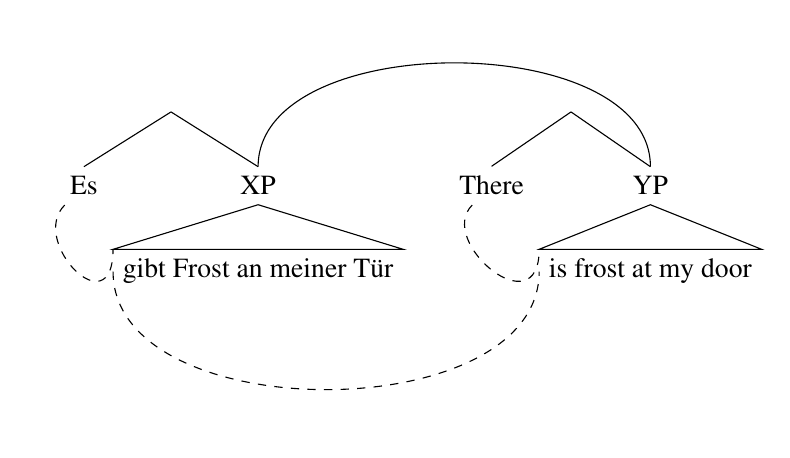
\begin{tikzpicture}
   \Tree [ [.\node(aDE){Es}; ]
    [.\node(pDE){XP};      
    \edge[roof]; \node(rDE){    gibt Frost an meiner Tür };  ] ] 
    \begin{scope}[shift={(2in,0in)}]
      \Tree [ [.\node(aEN){There};  ]
            [.\node(pEN){YP}; \edge[roof]; \node(rEN){ is frost at my door}; ] ]
          \end{scope}
          \draw[-] (pDE)..controls +(north:2) and +(north:2) .. (pEN); 
          \draw[dashed,-] (rDE.west)..controls +(south:2) and +(south:2) .. (rEN.west); 
          \draw[dashed,-] (aEN)..controls +(south west:1) and +(south:1) .. (rEN.north west); 
          \draw[dashed,-] (aDE)..controls +(south west:1) and +(south:1) .. (rDE.north west); 
\end{tikzpicture}
   \caption{N-gram-samanstilling versus syntaktiske frasar}
    \label{fig:ikkjenode}
  \end{figure}

Men sett no at me ikkje har som formål å nytte frasesamanstillinga til
reint N-grambasert omsetjing. Kva for \emph{lingvistiske} krav kan me
stille til å kalle to frasar samanstilte? Me må i alle fall tillate
ein del skilnad.  I alle større parallelltekster vil parallellstilte
setningar ha visse syntaktiske og semantiske\footnote{Sidan eg går ut frå at data er setningssamanstilt, kjem eg
       ikkje inn på diskurs-/pragmatiske verknader, med mindre dette
       fører til forskjellar innanfor setningane (sjå t.d. del
       \ref{SEC:ordkrav} om lenkjer mellom koreferente substantiv og
       pronomen). } omsetjingsskifte,
t.d. leksikalisering av syntaktiske konstruksjonar eller omvendt,
endring av ordklasse, presisering/depresisering, endringar i leksikale
trekk (t.d. telleleg/utelleleg),
osb. \citep[s.~56--62]{munday2001its}, slik at den einaste
fullstendige, «perfekte» samanstillinga vil vere
identitetsfunksjonen. Kor mykje mangel på samsvar me godtek blir då
avgjort av formålet med samanstillinga.

Eitt av formåla med samanstillinga i denne oppgåva er å kunne oppdage
korleis ulike språk realiserer semantiske roller syntaktisk; då
spesielt i forhold til hypotesane gitt i \citet[s.~7]{xpar2008rcn},
t.d. at «case marking might be useful to further determine a given
argument's semantic role». Skal me finne det siste, må me altså kunne
lenkje frasar med ulik kasusmarkering, men ha krav om lik tildeling av
semantiske roller; samtidig skal me sjå at me ikkje kan ha krav om lik
syntaktisk funksjon. I tillegg vil me sjølvsagt ikkje lenkje på tvers
av konstituentgrenser, sidan det er fullstendige konstituentar\footnote{LFG tillèt som nemnt diskontinuerlege konstituentar, men dette
        er ikkje det same som ikkje-konstituentar av typen «es gibt» /
        «there is». }
som fyller dei semantiske rollene.

Eit anna mogleg formål er å nytte desse frasesamanstillingane til
maskinomsetjing. \citet{riezler2006gmt} nyttar ein stokastisk
frasesamanstilling til å oppdage transfer-reglar for bruk i LFG-basert
generering i maskinomsetjing. Dette er reglar som omsett fragment av
ein f-struktur på kjeldespråket til f-strukturfragment på
målspråket. (Eit krav på utforminga av moglege transfer-reglar hindrar
at ein får reglar som lenkjar ikkje-konstituentar, eg kjem tilbake til
dette nedanfor.)  Samanstillinga utvikla her burde au kunne nyttast
til å finne slike transfer-reglar, men dette er ikkje noko eg har lagt
vekt på.

Nedanfor gir eg eit forslag til krav for frasesamanstilling, med desse
formåla i tankane. Om alle krava er moglege å implementere, er eit
separat problem.

\section{Frasesamanstilling i ein LFG-trebank}
\label{sec-3.3}


Samanstilte frasar bør ha nok semantisk likskap til å kunne opptre som
omsetjingar i liknande omgivnader
\citep[s.~74]{dyvik2009lmp}. \citet{thunes2003eal} gir nokre prinsipp
-- som er passande å ha som utgangspunkt -- for å fastslå det som kan
kallast \emph{omsetjingsmessig korrespondanse} (her for
ordsamanstilling). Dette er prinsipp som skal gjelde for eit litt
forskjellig formål, men som au «ligger nær opp til det vi intuitivt
mener er riktig» \citep[s.~2]{thunes2003eal}. Prinsippa blir nytta til
å lage ein gullstandard for ordsamanstilling\footnote{\cite[s.~2]{thunes2003eal}: «Våre prinsipper er satt
       opp for å tjene et bestemt formål, nemlig å samle inn data som
       metoden i Semantic Mirrors skal anvendes på», ein metode for å
       automatisk finne WordNet-liknande relasjonar frå
       parallelltekst. I denne metoden vil det vere naturleg med høge
       krav til presisjon, men kanskje lågare krav til dekning:
       speilmetoden skal finne leksikale semantiske forhold som held
       på \emph{typenivå}, medan for trebanken er det viktigare korleis me
       kan annotere eit \emph{token} av t.d. eit verb i ein viss VP i ei
       gitt korpussetning. },
hovudsakleg for dei opne klassene, og er definert ved å vise til kva
for rolle eit argumentord speler, eller kva for rolletildeling eit
predikat eller modifiserande ord gir. Så for å t.d. samanstille to
verb må dei ha like mange semantiske argument (men argumenta treng
ikkje alle realiserast syntaktisk) og dei må \emph{tildele same roller};
medan argumenta må \emph{spele same rolle}, og både argument og adjunkt må
vere \emph{koreferente}. Lenkja ord må vere del av frasar som speler same
rolle i «det som er felles i interpretasjonene av [dei to setningane]»
\citep[s.~3]{thunes2003eal}.

Viss me tek utgangspunkt i det siste, vil det vere naturleg å i
tillegg lenkje desse frasane som speler same rolle i «det som er
felles i interpretasjonene».

Krava for ordsamanstillinga må au vere fylt for at desse frasane kan
samanstillast. Ei ordsamanstilling er altså naudsynt for ein
frasesamanstilling, og omvendt. Dette er berre problematisk om me
føreset at det eine er derivert av det andre; men dette har me ingen
\emph{a priori} grunn til å gjere. Krava eg her utviklar bør i staden
sjåast på som \emph{skrankar} på moglege samanstillingar i modellen (jamfør
\ref{SEC:omgrepsavklaring} om modellteoretiske grammatikkar), heller
enn derivasjonelle forhold. Samtidig er det som nemnt eit mål å finne
ut kor uavhengig me kan gjere oss av ordlenkjingsinformasjonen (dette
er au nyttig for implementasjonen), utan at det treng å gi krava ei
\emph{retning}.

Ei frasesamanstilling er ei skildring av forhold mellom \emph{fragment} av
setningar, dette er endå ein grunn til at det er naturleg å skildre
dei ønskelege forholda som skrankar på moglege samanstillingar. Me kan
setje skrankar på f-struktur-, konstituent- og ordsamanstilling
samtidig, utan å måtte ha krav om at den eine samanstillinga er
fullstendig (eller delvis) avleiia av den andre, før me veit om eit
slikt avleiingsforhold er empirisk fundert. Me kan i tillegg ha
ufullstendige samanstillingar i dei tilfella der det er ufullstendig
samsvar mellom setningane (der ei fullstendig samanstilling ville
brutt visse krav).

Sidan metoden er mynta på bruk i ein LFG-parsa trebank, og delvis vil
nytte denne annotasjonen som datagrunnlag, er det naturleg å nytte
same konsept som blir nytta i LFG\footnote{I tillegg finst andre positive biverknader av ein LFG-basert
       frasesamanstilling for bruk i denne samanhengen, som at ein kan
       studere kor parallelle dei parallelle grammatikkane i
       ParGram-prosjektet \citep{butt2002pgp} faktisk er, på ulike
       nivå (leksikon og argumentstruktur, c-struktur, f-struktur). } (f-struktur, c-struktur,
endosentrisitetsprinsipp, \xbar{}-tre, osb.)  au i desse krava til den
«beste» frasesamanstillinga; i den grad LFG gir ein generaliserbar
skildring av syntaks, bør desse krava vere generaliserbare til andre
teoriar.

Utan skrankar i det heile vil alt kunne lenkjast til alt (noko som er
like unyttig som å ikkje lenkje noko); i del \ref{SEC:kandidatar} ser
eg på kva for typar element i dei lingvistiske analysane (ord,
grammatiske trekk, konstituentar, \ldots{}) det er fornuftig å tillate
lenkjer mellom. I avsnitta nedanfor spesifiserer eg kva som må til for
at me skal lenkje element av desse typane.

\section{Kva kan lenkjast?}
\label{sec-3.4}

\label{SEC:kandidatar}

Viss to uttrykk er samanstilt på setningsnivå (slik at me dimed kan gå
ut frå at dei er omsetjingar av kvarandre), og begge har ein
LFG-analyse, så har me iallfall tre ulike nivå kor me kan finne
ekvivalensforhold under setningsnivå:
\begin{enumerate}
\item mellom ord i setningane,
\item mellom f-strukturar,
\item mellom c-strukturnodar.
\end{enumerate}
På begge språk har me alle nivå -- det er ingen grunn til å lenkje på
tvers av nivå sidan forhold mellom desse nivåa er implisitt i
LFG-analysen.

Alle ord i setninga er \emph{kandidatar} for samanstilling med ord i
omsetjinga, men det kan godt hende at eit ord \emph{ikkje} har ei lenkje,
og me kan heller ikkje utelukke at det finst mange-til-mange-lenkjer
som ikkje kan «delast opp». Dette gjeld au nodane i c-strukturen.

Når det gjeld f-strukturane er det ganske mange element me teoretisk
sett kunne ha lenkja, t.d. enkelttrekk som kasus eller dei uordna
mengdene med adjunkt, men det som er mest \emph{nyttig} er nok å berre
lenkje der det er ei nær kopling til orda i setninga. Sidan alle
PRED-element i ein f-struktur unikt står for predikerande ord, kan me
-- gitt to samanstilte setningar -- la \emph{kandidatane for
samanstilling på f-strukturnivå} inkludere alle desse PRED-elementa i
f-strukturane til setningane\footnote{I del \ref{SEC:fnord} kjem eg tilbake til spørsmålet om me vil
        inkludere visse f-strukturar utan PRED-element i kandidatane
        for samanstilling. }. PRED-element representerer
semantiske bidrag som oftast er påkrevde på begge språk i omsetjingar,
medan andre f-strukturtrekk gjerne er valfrie på det eine av språka;
det er ikkje alle språk som har t.d. obligatorisk kasusmarkering, og
ein vil kanskje nytte trebanken til å oppdage nettopp slik variasjon.
\fxnote[inline,nomargin]{Diskutabelt, TODO:} PRED-elementa er i tillegg
gjerne enklare å knyte direkte opp mot den konkrete, observerte
tekststrengen, medan t.d. aspekt kanskje er umogleg å skilje frå
tempus i affikset.

Samtidig er det au eit omsetjingsforhold mellom trekka i same
f-struktur som dei lenkja PRED-elementa, og me ville kanskje ikkje ha
omsett dei to PRED-elementa i andre f-strukturkontekstar. Difor bør me
au sjå på ei PRED-lenkje som ei lenkje mellom \emph{f-strukturane til
desse PRED-elementa}\footnote{Eventuelt kunne me ha definert lenkjingskandidatane på
       f-strukturnivå som alle PRED-haldande f-strukturar, resultatet
       blir det same. }.  Med dette i tankane, kombinert med
c-struktur-f-strukturavbildinga $\phi$ (sjå del
\ref{SEC:omgrepsavklaring}), får me følgjande samanheng, illustrert i
figur \ref{fig:viss-PRED-så-f-og-c}:

\ex. \label{f-links} Ei lenkje mellom to PRED-element $p$ og $q$, kor
      $p$ er medlem av f-strukturen $f$, og $q$ er medlem av
      f-strukturen $g$, tilseier at:
\a. \label{f-links-substr} me tolkar f-strukturane $f$ og $g$ som lenkja,
\b. \label{f-links-words} orda i setningane som projiserer
     PRED-elementa tek del i ei lenkje (kor andre
     ord kan vere involvert), og at
\c. \label{f-links-domain} iallfall dei øvste nodane i $\phi^{-1}(f)$
     og $\phi^{-1}(g)$, dei funksjonelle domena til f-strukturane $f$
     og $g$, er lenkja 

  \usetikzlibrary{calc}
  \begin{figure}[htp]
    \begin{tikzpicture}
    {\avmoptions{}
     \node(src){
        \begin{avm}
          $f$ \[pred  & `{\bf{}sove}<jeg>' \\
          tense & pret \\
          ... \]
        \end{avm}
      };
      \node[right of=src, node distance=5cm](trg){
        \begin{avm}
          $g$ \[pred   &  `{\bf{}sleep}<I>'\\
          tense  & pret  \\
          aspect & simple \\
          ... \]
        \end{avm}
      };
      }
      \draw[dashed,-] (src.west) .. controls +(-1,2) and +(-1,2) .. node[above,sloped]{$l_f$} (trg.west) ;
      \draw[-] ($(src.north)-(1,0.3)$) .. controls +(0,1.5) and +(0,1.5) .. node[above,sloped]{$l_p$} ($(trg.north)-(1,0.3)$) ;

      \begin{scope}[shift={(0,-3cm)}]
     \Tree  [.\node(VPs){VP}; [.\node(Vs){V}; \node(sov){sov};  ] ]
      \begin{scope}[shift={(5cm,0)}]
        \Tree  [.\node(VPt){VP}; [.\node(Vt){V}; \node(slept){slept};  ] ]
      \end{scope}
      \end{scope}
      \draw[-] (VPs)..controls +(north:1.5) and +(north:1.5) .. node[above,sloped]{$l_c$} (VPt) ;
      \draw[dashed,-] (sov)..controls +(north east:1.5) and +(north west:1.5) .. node[above,sloped]{$l_o$} (slept) ;
   \end{tikzpicture}
    
\fxnote{TODO: teikne inn f-domene}

    \caption{Ei PRED-lenkje $l_p$ kan tolkast som ei f-strukturlenkje
    $l_f$, og impliserer ei c-strukturlenkje $l_c$ mellom toppnodane i
    dei funksjonelle domena. Orda som projiserer PRED-elementa er med
    i ei lenkje $l_o$ (som kan inkludere fleire ord).}
   \label{fig:viss-PRED-så-f-og-c}
 \end{figure}

Punkt \ref{f-links-substr} og \ref{f-links-domain} over seier at viss
PRED-elementa projisert av t.d. to verb i verbfrasar er lenkja, vil
VP-ane som heilskap vere lenkja (både VP-nodane som dominerer dei
lenkja funksjonelle domena, og f-strukturane frå ytre PRED til verba),
det er dette at heile VP-ane er lenkja som gjer det til ei fraselenkje
og ikkje berre ei ordlenkje. Punkt \ref{f-links-substr} er forsvart
over, medan punkt \ref{f-links-domain} kjem som ein konsekvens av at
øvste node dominerer alle nodar i det funksjonelle domenet; det er det
funksjonelle domenet som spesifiserer informasjonen i f-strukturane,
toppnodane dominerer heile dette domenet og bør difor lenkjast viss og
berre viss f-strukturane er lenkja.  

Alle nodar i c-strukturen (alle syntaktiske \emph{frasar/konstituentar} i
setninga) som kan koplast til PRED-haldande f-strukturar, vil vere
kandidatar for samanstilling på c-strukturnivå (dette inkluderer
diskontinuerlege konstituentar), men ikkje alle vil bli lenkja.  I del
\ref{SEC:subnode} ser eg på kva som må til for å lenkje ikkje-øvste
nodar i det funksjonelle domenet.
I tillegg finst det nodar over ord som ikkje projiserer PRED-element,
desse kjem eg tilbake til i del \ref{SEC:fnord}.

I følgje punkt \ref{f-links-words} vil fraselenkja leie til at sjølve
verba i to lenkja VP-ar au er lenkja, som tilseier at \emph{ei PRED-lenkje impliserer ei ordlenkje}. I visse tilfelle er dette heilt
uproblematisk, t.d. viss \emph{I slept down by the river} skal lenkjast med
\emph{Eg sov nede med elva} vil me uansett lenkje \emph{slept} og \emph{sov}; dette
kan gjelde transitive verb au:

\ex. \a. The locusts have no king, just noise and hard language\\
     $\leftrightarrow$
     \b. Grashoppene har ingen konge, berre støy og krasse ord

\fxnote{der ADJUNKT ikkje er realisert, lenkjer me ikkje PRED.  skal
me då ikkje lenkje ord heller?}

\fxnote{finst det tilfelle der ordlenkjer ikkje impliserer PRED-lenkjer? 
\\
(hypotese: det er alltid slik at ordlenkjing av predikerande ord => PRED-lenkje)
\\
PRED->ord :: iallfall\\
PRED<-ord :: ?\\
PRED<->ord\\
PRED, ord}

\emph{have/har} tek del i VP-samanstillinga \emph{have no king.../har
ingen konge...}, her au skal det vere uproblematisk å lenkje
enkeltorda \emph{have} og \emph{har}.

Men som nemnd treng ikkje ordsamanstillinga vere ein-til-ein, det
punkt \ref{f-links-words} seier er at desse orda iallfall er ein del
av ein samanstilling med kvarandre (i døme \Last altså
VP-samanstillinga). Kanskje er dette ei mange-til-mange-lenkje som
ikkje \emph{kan} reduserast til ein-til-ein-lenkjer; eller kanskje er
det som i \Last mogleg å skilje ut delsamanstillingar, som
\emph{have/har}. Eg kjem tilbake til dette
\fxnote[inline,nomargin]{TODO: når?} seinare.

Sidan PRED-lenkjing impliserer ordlenkjing, må me sjekke om krava på
ordnivå (del \ref{SEC:ordkrav}) er oppfylte for å lenkje to
PRED-element. \fxnote{TODO: litt brå avslutning}

\section{Krav på ordnivå}
\label{sec-3.5}

\label{SEC:ordkrav}

Ord som skal lenkjast må i \cite{thunes2003eal} vere del av frasar som
speler same rolle i det som er felles i interpretasjonane, her kan me
omskrive det til at dei må vere del av \emph{frasar som er lenkja på c-strukturnivå}; forholda i \ref{f-links} gir då koplinga til krav på
andre nivå (t.d. vil krav om tildeling av like mange roller vere
meir passande å spesifisere på f-strukturnivå).

Det er visse ting me ikkje kan spesifisere ut frå rein c- og
f-strukturinformasjon. Den norske setninga \emph{eg vil ete} kan fint
samanstillast med \emph{I want to eat}, med ei lenkje mellom \emph{ete} og
\emph{eat}. Men kva står i vegen for å lenkje \emph{ete} til hovudverbet i \emph{I want to drink}? Forskjellen på f-strukturnivå er berre at PRED-verdien
er ulik (\textbf{eat} mot \textbf{drink}). Me må altså ha eit krav om at tydinga til
lenkja ord (og deira predikat) er «lik nok» til at me kan sjå på dei
som omsetjingar\footnote{Eigentleg burde slike setningar ikkje vere lenkja på
        setningsnivå ein gong, men som me skal sjå i del
        \ref{SEC:lik-argstr} treng me kravet om lik tyding 
        sjølv innanfor setninga. }. \citet[s.~74]{dyvik2009lmp} krev dei at orda
generelt, utan kontekst, må vere semantisk plausible omsetjingar,
eller at målordet er eit medlem av mengda av \emph{linguistically predictable translations} av kjeldeordet. Målordet har då
\emph{LPT-korrespondanse} med kjeldeordet. Informasjon om slik
LPT-korrespondanse kan komme frå ei djup semantisk dekomponering av
kvart ord, då blir det eit krav på f-strukturnivå (eller på ein
semantisk struktur), eller han kan komme bottom-up, typisk frå
automatisk ordsamanstilling. Bottom-up-informasjonen viser då om orda
generelt (i ulike kontekstar) blir nytta som omsetjingar av kvarandre.
Nedanfor reknar eg LPT-kravet som eit krav på ordnivå.

\fxnote{TODO: Er det mogleg å presisere LPT-kravet meir? Skal det
berre vere eit rangeringskrav??}
 
Ein type presisering/depresisering (del \ref{SEC:formaal}) me ofte ser
i omsetjingar er at eit pronomen på kjeldespråket blir nytta der
målspråket har eit koreferent substantiv, eller
omvendt. \citet{dyvik2009lmp} opnar for at desse au har
LPT-korrespondanse (som nemnt i \cite{thunes2003eal} må lenkja ord
uansett vere koreferente).

Men kva då med lenkjing av pronomen til verb bøygd for person og tal i
pro-drop-språk?

\ex. \a. iqePa                                  \hfill{} (georgisk) \\
     $\leftrightarrow$
     \b. han bjeffa

Viss setningane i døme \Last er lenkja, der iqePa har eit pro-argument
koreferent med \emph{han} som subjekt, bør dei to subjekta iallfall kunne
lenkjast på f-strukturnivå; dei har same referent og speler same rolle
i argumentstrukturen til verba (som me går ut frå er lenkja). På
ordnivå, derimot, kan me ikkje lenkje \emph{han} til \emph{iqePa} åleine -- her
må me ha ei mange-til-ein-lenkje mellom $\{ \rm han, bjeffa \}$ og $\{
\rm iqePa \}$. 
Generelt må me ha slike lenkjer der eitt ord projiserer fleire
PRED-element\footnote{Me ville au fått ei mange-til-ein-lenkje om me tillot
        \emph{komplekse predikat} i analysane, t.d. slik
        \citet{butt1998merger} foreslår ved å la kombinasjonen av to
        ord endre argumentstrukturen til eitt PRED-element. }.

\subsection{Ordklasse}
\label{sec-3.5.1}

Ulike språk leksikaliserer same konsept på ulike
måtar. \citet[s.~3]{cheung2002scg} nemnar vanskane med å ha eit krav
om lik ordklasse i utviklinga av ein kinesisk-engelsk termbank, kor
t.d. det engelske ordet \emph{fulfilment} meir naturleg blir omsett til eit
verb på kinesisk. På same måte vil eit georgisk verbalsubstantiv
(\emph{masdar}) gjerne bli omsett til eit verb i infinitiv på
norsk. Slike skifte mellom ordklasser er svært vanlege i
omsetjing\footnote{\citet[Catford~(1965),~i][s.~61]{munday2001its} gir ein gjennomgang av
       slike \emph{klasseskifte}, og andre typar omsetjingsskifte. }.

Me kan opne for ordklasseoverskridande lenkjer der det er samsvar på
andre nivå, me bør iallfall krevje ein likskap i argumentstruktur; så
om LPT-kravet og krava på c- og f-strukturnivå er fylt, bør det ikkje
vere noko i vegen for å lenkje ord (eventuelt mengder av ord) av ulik
ordklasse.

\section{Lenkjing av underordna c-strukturnodar}
\label{sec-3.6}

\label{SEC:subnode}

Toppnodane i eit lenkja funksjonelt domene i c-struktur (XP på språk
1, ZP på språk 2) vil ha ein informasjonsmessig korrespondanse, og kan
samanstillast. Men det er mogleg å samanstille to toppnodar i
funksjonelle domene i c-strukturen utan at nodane under (X', Z') er
samanstilt. Ein grunn til å ikkje samanstille desse underordna nodane,
vil vere viss spesifikator til X ikkje speler same rolle i tolkinga
som spesifikator til Z, dvs. viss YP og WP i figur \ref{fig:subnode}
ikkje er lenkja.


Me kan utelukke lenkjing av ikkje-konstituentar som \emph{there is} ved å
krevje at ei fullstendig samanstilling mellom to frasar må vere slik
at heile substrukturen au er samanstilt. \emph{There is} og \emph{Es gibt} i
figur \ref{fig:ikkjenode} kan då ikkje samanstillast åleine, men berre
som del av ei ytre frasesamanstilling.
Så når \emph{kan} me samanstille nodane som står under øvste node i
det funksjonelle domenet?

\begin{figure}[htp]
   \vfill{} % how todo?
   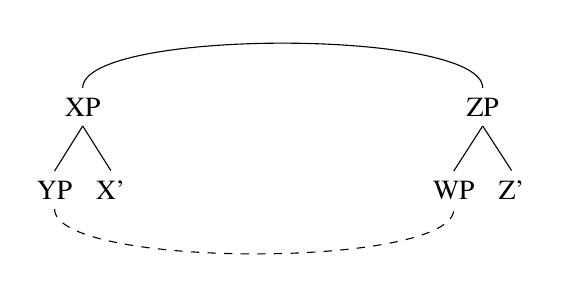
\begin{tikzpicture}
  \Tree  [.\node(XP){XP};  \node(YP){YP};  
                                    \node(X'){X'};   ]
      \begin{scope}[shift={(2in,0in)}]
  \Tree  [.\node(ZP){ZP};  \node(WP){WP};  
                                    \node(Z'){Z'};   ]
\end{scope}
\draw[-] (XP)..controls +(north:1) and +(north:1) .. (ZP) ;
  \draw[dashed,-] (YP)..controls +(south:1) and +(south:1) .. (WP) ;

\end{tikzpicture}
   \caption{Lenkjing av underordna c-strukturnodar}
   \label{fig:subnode}
  \end{figure}

I figur \ref{fig:subnode} der XP og ZP er lenkja, vil YP og WP -- i
kraft av å vere toppnodar i sine domene -- måtte ha ei lenkje i
f-strukturen for at c-strukturnodane kan lenkjast (det kunne jo
t.d. hende at f-strukturen projisert av YP samsvarte med den projisert
av Z', eller ein struktur under Z').

Om me skal lenkje Z' og X' i figuren over må dei respektive
spesifikatornodane vere lenkja. Me får då følgjande krav:

\ex. \label{subnodekrav} Krav for lenkjing av underordna
c-strukturnodar:
\a. c-strukturnodar som ligg under øvste node i to funksjonelle
    domena kan berre samanstillast med nodar som ligg innanfor desse
    domena,
\b. c-strukturnodar kan berre samanstillast om deira funksjonelle
    domene er lenkja på f-strukturnivå,
\c. om ein c-strukturnode X' som ikkje er toppnode i det funksjonelle
    domenet har ein søsternode YP, må YP vere samanstilt med ein
    søsternode til Z' for å samanstille X' og Z'


\Last[a] seier at om XP og ZP er samanstilt, der XP er t.d. OBJ til
IP, kan ikkje Z' samanstillast med SUBJ til IP osb., men berre til
nodar innanfor OBJ-domenet. \Last[c] påført figur \ref{fig:subnode}
seier altså at spesifikatornodane må vere lenkja for at X' og Z' skal
lenkjast (manglande søsternode på den eine sida vil au hindre
samanstilling).

I figur \ref{fig:fnord} er alle nodane under S vist i dei to trea i
same funksjonelle domene (kvar node under S er annotert med $\uparrow
= \downarrow$), så om dei funksjonelle domena er samanstilt (som krev
at \emph{rom cvimda} og \emph{at det regner} er samanstilt), vil \Last[a og -b]
vere oppfylt kva gjeld CP-komplementa -- lenkjinga går ikkje ut over
dei funksjonelle domena. Sidan Csub og Cnom er funksjonelle kategoriar
er dei au samanstilt via samanstillinga av S-nodane og føringane i
\ref{fnordkrav}, og \Last[c] er då oppfylt. \Last står altså ikkje i
vegen for å samanstille IP-en over \emph{cvimda} og Ssub.

I figur \ref{fig:ikkjesub} derimot \citep{mrs-suite}, kan me ikkje
samanstille I'-nodane. PRONP-noden, spesifikator på den norske sida,
er ikkje lenkja med nokon spesifikator på den georgiske sida. Den
informasjonen (her reint syntaktisk) som ordet \emph{det} tilfører IP, ligg
under I' på georgisk. Om me skulle lenkja I', måtte me altså hatt ein
georgisk spesifikator som var lenkja til den norske PRONP.

\begin{figure}[htp]
 \vfill{} % how todo?
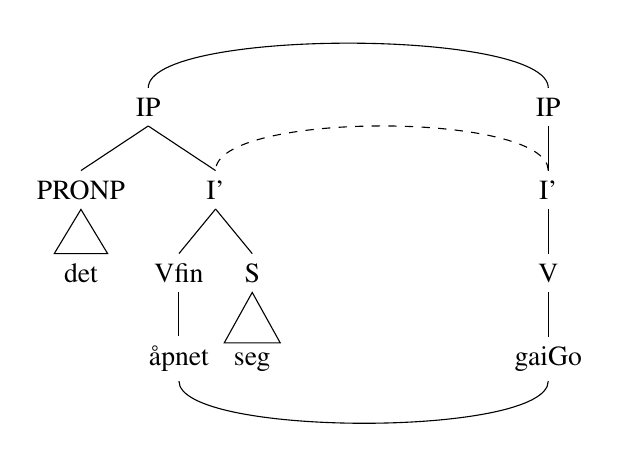
\begin{tikzpicture}
\Tree [.\node(IPb){IP}; 
  [.PRONP \edge[roof]; {det} ] 
  [.\node(Ibarb){I'};  [.Vfin \node(åpnet){åpnet};  ]
       [.S \edge[roof]; {seg} ] ] ]
      \begin{scope}[shift={(2in,0in)}]
\Tree [.\node(IPk){IP}; 
  [.\node(Ibark){I'};  [.V    \node(gaiGo){gaiGo};  ]
  ] ]
\end{scope}
 \draw[-] (IPk)..controls +(north:1) and +(north:1) .. (IPb) ;
  \draw[dashed,-] (Ibark)..controls +(north:1) and +(north:1) .. (Ibarb) ;
 \draw[-] (gaiGo)..controls +(south:1) and +(south:1) .. (åpnet) ;

\end{tikzpicture}
\caption{Umogleg samanstilling av funksjonsord mellom bokmål og georgisk}
 \label{fig:ikkjesub}
\end{figure}

\section{Funksjonsord}
\label{sec-3.7}

\label{SEC:fnord}
I tillegg kan me ha ord i setninga som ikkje tilsvarer PRED-element i
f-strukturen, typisk funksjonsord (t.d. \emph{som}, \emph{at}). Ved
endosentrisitetsprinsippa til \citet{bresnan2001lfs} er komplementet
til funksjonelle kategoriar (C, I, P) ein funksjonell ko-kjerne. 

\ex. \label{fnordkrav} Skal nodar for ord som ikkje projiserer
     PRED-element\footnote{Skal ein lenkje ordet \emph{som} (utan PRED) med ordet \emph{which} (med
        PRED)? Viss begge står under C i treet, kan det kanskje vere
        informativt med ein type «defekt» lenkje, sjølv om berre det
        eine ordet blir rekna for å vere eit innhaldsord. Frasane til
        deira funksjonelle domene vil uansett vere samanstilt via
        toppnodane (t.d. CP). } samanstillast, må følgjande krav vere oppfylt:
\a. det funksjonelle domenet (gitt ved komplementet) må vere
   samanstilt, og
\b. dei er begge c-strukturhovud.


Om \Last[a og -b] er oppfylt, kan me få samanstillinga vist i figur
\ref{fig:fnord}, og i dette tilfellet er \Last[b] oppfylt og \Last[a]
vil vere oppfylt om me kan samanstille \emph{cvimda} med \emph{det regnet}.

  \begin{figure}[htp]
   \vfill{} % how todo?
  
  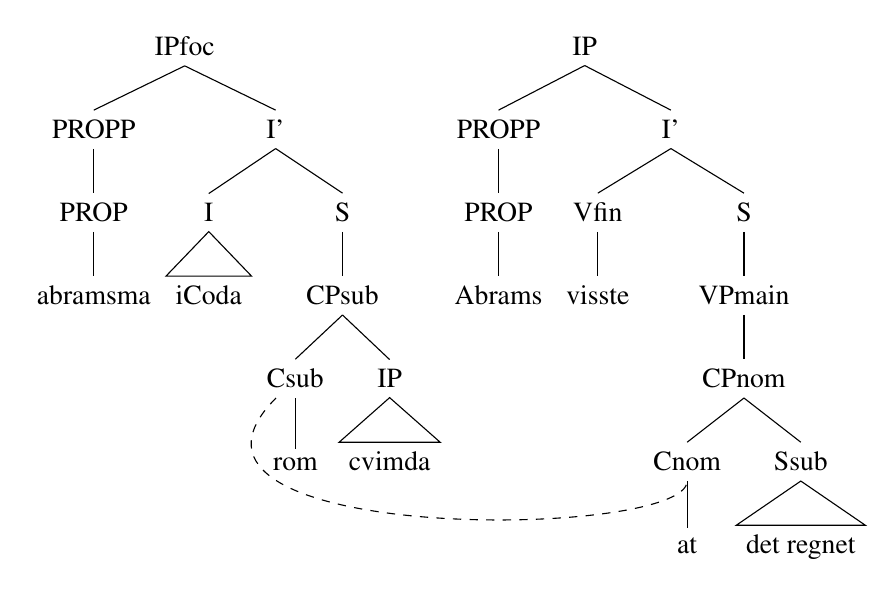
\begin{tikzpicture}
  \Tree
  [.IPfoc
    [.PROPP [.PROP abramsma ] ] 
    [.I' [.I \edge[roof]; {iCoda} ]
             [.S [.CPsub
                  [.\node(Csub){Csub};  rom ]
                  [.IP \edge[roof]; {cvimda} ]]]]]
      \begin{scope}[shift={(2in,0in)}]
  \Tree
  [.IP
    [.PROPP [.PROP Abrams ] ]
     [.I' [.Vfin visste ]
              [.S [.VPmain [.CPnom
                           [.\node(Cnom){Cnom};  at ] 
                            [.Ssub \edge[roof]; {det regnet} ]]]]] ]
  \end{scope}                      
  \draw[dashed,-] (Csub)..controls +(south west:3) and +(south:1) .. (Cnom) ;
  \end{tikzpicture}
  \caption{Mogleg samanstilling av funksjonsord mellom georgisk og norsk (bokmål)}
   \label{fig:fnord}
  \end{figure}

\section{Krav om lik argumentstruktur}
\label{sec-3.8}

\label{SEC:lik-argstr}

\citet{thunes2003eal} gir som nemnd eit krav om at \emph{predikat må ha tilsvarande semantiske argument} for å samanstillast.

Om det alltid er slik at to predikat har like mange argument, som kjem i
same rekkjefølgje i argumentstrukturen, vil det gjere den praktiske
oppgåva med å samanstille predikata, og argument med argument, mykje
enklare. Men kan me stille så sterke krav?

Sett at ein setning på språk 1 har ei \emph{at}-setning som adjunkt, medan
denne setninga på språk 2 er eit argument, og at desse setningane
ville vore samanstilte om dei opptredde åleine. Om dei uttrykkjer same
proposisjon og \emph{speler same rolle i verbsituasjonen},
synest det naturleg å lenkje desse.  

Omsetjingsrelasjonar gir data for verbsituasjon, på eit meir generelt
grunnlag enn det me kan få frå einspråklege analysar åleine. Om me har
gode semantiske grunnar for å kalle ein deltakar i ein verbsituasjon
eit argument på eitt språk, vil dei same grunnane gjelde for
omsetjingsmessig korresponderande verb på andre språk. Ein kan då
nytte unionen over alle argument til korresponderande verb til å
karakterisere kva ein meiner med \emph{deltakarane i verbsituasjonen}. Syntaktiske forhold i språket kan sjølvsagt gi
grunnar til å \emph{ikkje} kalle dette eit argument (om det er mogleg å
finne akseptable syntaktiske grunnar for å kalle noko ein adjunkt
heller enn eit argument).
 
For å gjere dette konkret kan me sjå på setning 7 i MRS-suiten
\citep{mrs-suite}\footnote{Setningane i første og tredje linje i døma er direkte henta frå
       MRS-suiten, med mindre anna er opplyst. }:

\exg.  abramsi brouns       daenajleva sigaretze, rom cvimda \\
      Abrams.NOM Brown.DAT vedde.3SG sigarett.om, at  regne.3SG.IMP \\
     `Abrams veddet en sigarett med Brown på at det regnet' 

I følgje LFG-parsen til desse setningane har hovudpredikata svært ulik
argumentstruktur\footnote{Analysane er henta 18. mai, 2009, frå
        \href{http://decentius.aksis.uib.no/logon/xle.xml}{http://decentius.aksis.uib.no/logon/xle.xml}, som implementerer
        LFG-grammatikkane frå ParGram-prosjektet \citep{butt2002pgp}. }. Det norske \emph{vedde} har \underline{fire} argument, medan
\emph{da-najleveba} har \underline{to} (\emph{Abrams} og \emph{Browne}), kor at-setninga på
norsk og \emph{rom cvimda} uttrykkjer same proposisjon og speler same rolle
i verbsituasjonen. Den engelske LFG-parsen av den tilsvarande setninga
(mine omsetjingar) gir \underline{tre} argument, \emph{with} blir her adjunkt, medan
den tyske grammatikken, som au har \underline{tre} argument, gjer \emph{at}-setninga
til adjunkt. I \Next nedanfor har eg representert dei omsetjingsmessig
korresponderande frasane i f-strukturane med dei norske omsetjingane
for å illustrere dette:

{\avmoptions{}
\ex. \label{vedde}
\a. Adams veddet en sigarett med Browne \hfill{} (norsk bokmål)\\ på at det regnet.\\
    $\\\begin{avm}\[pred & `{\bf{}vedde}<Abrams, sigarett, Browne, regne>' \\
                 adjunct & \{\}\]\end{avm}\\$
\b. abramsi brouns daenajleva sigaretze, rom cvimda. \hfill{} (georgisk)\\
    $\\\begin{avm}\[pred &  `{\bf{}da-najleveba}<Abrams, Browne, regne>'\\
    adjunct &  \{ \rm sigarett \}\]\end{avm}\\$ 
\c. Abrams hat mit Browne um eine Zigarette gewettet, \hfill{}(tysk)\\
    daß es regnet.\\
    $\\\begin{avm}\[pred & `{\bf{}wetten}<Abrams, sigarett>' \\
                  adjunct & \{ \rm Browne, sigarett \}\]\end{avm}\\$
\d. Abrams bet a cigarette with Brown that it was raining. \hfill{}(engelsk)\\
    $\\\begin{avm}\[pred & `{\bf{}bet}<Abrams, sigarett, regne>'\\
                  adjunct & \{ \rm Browne \}\]\end{avm}$

}

Om ein skal ha grammatikkane som datagrunnlag er det altså eit reellt
problem kva ein skal gjere med mangel på samsvar i
argumentstruktur. Om det alltid var fullstendig samsvar i
argumentstruktur, ville det vore trivielt å lenkje argument: viss to
korresponderande verb hadde tre argument, ville me lenkja det første
med det første, det andre med det andre og det tredje med det
tredje. Men om me har analysar som dei over, ser det ut til at me
treng bottom-up-informasjon om kva for adjunkt og argument som
samsvarer.

Det same gjeld forøvrig lenkjing av adjunkt til adjunkt. Adjunkt
plukker ut si eiga rolle der argument får rolla tildelt frå verbet, og
f-strukturane har ingen hierarkisk inndeling av desse slik me har for
verb og argument, dei er i staden representert som \emph{uordna mengder}.

\subsection{\textbf{TODO} Sitere eigen korpusundersøking av variasjon i arg-str?}
\label{sec-3.8.1}

Ei undersøking av den frasesamanstilte trebanken SMULTRON
\citep{samuelsson2006pap} mot LFG-grammatikkane for engelsk og tysk
fann at 2 av 15 korresponderande verbtoken\footnote{25 om ein inkluderer analysar kor minst eitt av argumenta
        ikkje hadde korrekt analyse (t.d. eit \textsc{PRO} der
        grammatikken burde funne eit substantiv). } for høgfrekvente
innhaldsverb fekk analysar kor argument korresponderte med adjunkt
\citep{unhammer2009aaa}.

\fxnote{LCS, dorr}
\subsection{\textbf{TODO} Ulik følgje i argumentstruktur}
\label{sec-3.8.2}

I tillegg til at argument kan lenkjast til adjunkt, kan koreferente
argument ha ulik følgje i argumentstrukturen. Det er klart at me vil
lenkje objektet til \emph{gefallen} (eller bokmål: \emph{behage}) med subjektet
til \emph{like}, og omvendt.  Men rekkjefølgje i argumentstrukturane i
ParGram-prosjektet er ofte basert på syntaktisk funksjon heller enn
rolle, slik at eit verb som har opplevar som objekt og tema som
subjekt vil ha opplevar nedanfor tema i argumentstrukturen, medan ei
omsetjing av dette verbet kan ha tema nedanfor:

{\avmoptions{}
\ex. \a. sie$_j$ gefallen ihnen$_i$ \\
     $\begin{avm}\[pred & `{\bf{}gefallen}<de$_j$, de$_i$>' \]\end{avm}$
    $\\\\\leftrightarrow$\\
     \b. de$_i$ liker dem$_j$ \\
     $\begin{avm}\[pred & `{\bf{}like}<de$_i$, de$_j$>' \]\end{avm}$

}

Argumentstrukturane i \Last har omvendt intern følgje, og som vist ved
dette dømet er det heller ikkje noko f-strukturinformasjon me kunne
nytta til å sikre lenkjinga \emph{sie/dem} og \emph{ihnen/de}. Igjen ser det ut
til at bottom-up-informasjon trengst.



\section{\textbf{SKRIV} Kan adjunkt lenkjast til nodar \underline{under} mor-lenkja?}
\label{sec-3.9}

\label{SEC:merge-daughters}

Krav (vi) i \citet[s.~75]{dyvik2009lmp} krev at viss F$_s$ og F$_t$ er
lenkja, så kan ingen adjunkt D$_s$ til F$_s$ vere lenkja til nodar utanfor
F$_t$. Men kan ein D$_s$ lenkjast til ei dotternode av argument eller
adjunkt til F$_t$?

R$_t$ er dotter til F$_t$, og må då vere lenkja til ei dotter av F$_s$,
A$_s$. Då må au alle argument til R$_t$ vere lenkja til døtre av A$_s$, så
D$_s$ kan ikkje lenkjast til argument av dotternodar til F$_t$. Kva med
adjunkt? Om me finn eit ulenkja adjunkt til R$_t$ kan me heller ikkje
lenkje dette til D$_s$ ved krav (vi) igjen, sidan D$_s$ står utanfor
A$_s$.

Men om D$_t$ er ei ulenkja \emph{adjunkt}dotter av F$_t$, så vil døtre av
D$_t$ kunne lenkjast til D$_s$, så lenge D$_t$ forblir ulenkja. Me kan altså
sjå ned i adjunktdøtre av F$_t$ for å lenkje D$_s$. 

På same måte bør ein kunne rekursivt sjå ned i ulenkja adjunktdøtre av
R$_t$, men ein bør kanskje ikkje kunne lenkje så djupt uansett? Ikkje
automatisk, uansett.



Programmet mitt vil, gitt to initielle f-strukturar med
LPT-korrespondanse, finne alle moglege kombinasjonar av lenkjer som
inneheld alle argument og kanskje adjunkt, dvs. om me har

\begin{verbatim}
 F_s [ PRED p<1,2> ADJUNCT { 3 } ]
\end{verbatim}


\begin{verbatim}
 F_t [ PRED p<4> ADJUNCT { 5,6 } ]
\end{verbatim}


vil dette vere logisk moglege samanstillingar av «f-strukturdøtre»:

\begin{verbatim}
    (((1 . 4) (2 . 5)) ((1 . 4) (2 . 6)) ((1 . 5) (2 . 4))
     ((1 . 5) (2 . 6) (3 . 4)) ((1 . 6) (2 . 4)) ((1 . 6) (2 . 5) (3 . 4)))
\end{verbatim}


Me luker ut kombinasjonar som bryt med LPT-korrespondanse. Med full
informasjon bør me sjølvsagt berre ende opp med éin kombinasjon,
t.d. \texttt{((1 . 4) (2 . 5))}.

Så langt bør altså krav (i-iv) frå \citet{dyvik2009lmp} vere dekkja.

Me \underline{kan} krevje at f strukturane-til f strukturdøtre-kan lenkjast
rekursivt for at F$_s$ og F$_t$ skal lenkjast, t.d. både \texttt{(1 . 4)} og \texttt{(2 . 5)}. Men her kjem det (iallfall) to problem.


\subsection{1. Kausativar og inkorporering}
\label{sec-3.9.1}

Om me har 

\begin{verbatim}
 F_s [ PRED p<SUBJ, 1, 2> XCOMP 2[ PRED q<1> ] ]
\end{verbatim}


\begin{verbatim}
 F_t [ PRED pq<SUBJ,OBJ> ]
\end{verbatim}


kor pq er t.d. ein kausativ som tilsvarer \texttt{p<..., q>}, så vil me ikkje
kunne lenkje F$_s$ og F$_t$ sidan det bryt med krav (iii), F$_s$ har eit
argument for mykje. Men her vil det kanskje vere naturleg å ha ei
ein-mange-lenkje:

\begin{verbatim}
 ((F_s 2) . F_t)
\end{verbatim}


No kan me sjå på unionen av argument av F$_s$ (minus XCOMP) og argument
av XCOMP, alle argument i denne unionen må då ha LPT-korrespondanse
med argument/adjunkt av F$_t$, og alle argument av F$_t$ må ha
LPT-korrespondanse med argument/adjunkt av unionen.

Det same bør kanskje skje ved vanleg inkorporering av substantiv, då
må det altså vere mogleg å føye saman t.d. verb og objekt; ein
kombinasjon av dette og kausativ bør vel vere mogleg, t.d.

\begin{verbatim}
 F_s [ PRED la<SUBJ, 1>  XCOMP 2[ få<1, 3:pengar> ] ]
\end{verbatim}


\begin{verbatim}
 F_ t [ PRED belønn<SUBJ, 1> ]
\end{verbatim}


Igjen ser me på argument frå unionen av \texttt{(F\_s 2 3)} minus 2 og 3, og
om det er mogleg å lenkje dei til argument/adjunkt av F$_t$, og omvendt.

Men det bør kanskje vere grenser for kor langt samanføying kan gå… eg
kan ikkje tenkje meg at me vil lenkje \texttt{((F\_s 2) . F\_t)} eller \texttt{((F\_s 1 2) . F\_t)} her:

\begin{verbatim}
 F_s [ PRED p<…, 1> XCOMP 1[ PRED q<…, 2> XCOMP 2[ PRED r<…> ] ] ]
\end{verbatim}


\begin{verbatim}
 F_t [ PRED pr<…> ]
\end{verbatim}


\ldots{}men det kan jo hende det finst situasjonar der dette au vil vere
rett. Problemet er altså kor me skal setje grensene i
implementasjonen. Om me skal prøve å samanføye på alle moglege måtar
(altså, der me ikkje har informasjon om LPT), i tillegg til «vanlege»
lenkjer, blir det fort komputasjonelt vanskeleg. Me kan sjølvsagt snu
på LPT-kravet her, og seie at dette er berre lov der me har positiv
informasjon om LPT-korrespondanse, i staden for at det ikkje er lov om
me har motstridande LPT-informasjon, det vil nok hjelpe, men det er
vanskeleg å finne prinsipelle avgrensingar her. 
\subsubsection{\textbf{TOGROK} adjunkt bør ikkje samanføyast? eller?}
\label{sec-3.9.1.1}

Det einaste eg kan
tenkje meg er at adjunkt ikkje bør vere kandidatar for samanføying (i
såfall burde dei vel heller vore analysert som argument?).

\subsection{2. Adposisjonsobjekt}
\label{sec-3.9.2}


I følgjande setningspar har me eit objekt «sigarett» som svarer til
PP-en «sigaretze» («sigareti» + «ze»), eit adjunkt:

\begin{verbatim}
 Abrams veddet en sigarett med Browne på at det regnet.
 abramsi brouns daenajleva sigaretze, rom cvimda.
\end{verbatim}


\begin{verbatim}
 F_s [ PRED sigarett ]
\end{verbatim}


\begin{verbatim}
 F_t [ PRED ze<1> 1[ PRED sigareti ] ]
\end{verbatim}


F$_s$ og F$_t$ er døtre av dei ytre predikata i kvar setning, krav (iii)
seier at det må vere LPT-korrespondanse mellom desse for at me skal
kunne lenkje «veddet» og «daenajleva».  Her synest det feil å føye
saman «sigareti» og «ze», \texttt{(F\_s . (F\_t 1))}, sidan «sigarett» ikkje
inneheld informasjonen gitt av «ze».

Det finst då to løysingar. Me kan slakke på LMT-kravet ved å la
\texttt{L'(F\_t) = \{sigaretze, ze\}} (evt. \texttt{\{sigaret, ze\}}), då kan me lenkje
\texttt{(F\_s . F\_t)}, medan 1 er ulenkja.

Eller me kan lenkje \texttt{(F\_s . 1)}, kor me har skikkeleg
LMT-korrespondanse, men då må me slakke på (iii) og (iv), og altså ha
lov til å «hoppe over» ein f-struktur for å lenkje «veddet» og
«daenajleva». F$_t$ er då ulenkja. Det er løysinga valt i
\citet[s.~75,~fotnote~3]{dyvik2009lmp}, og den løysinga eg følgjer
nedanfor.

\section{\textbf{TODO} Konstruksjonar og komposisjonell inekvivalens}
\label{sec-3.10}

\xbar-teori føreset at det finst éi dotter i kvart ledd som kan
reknast som predikatet for dette leddet. Ei utfordring for
\xbar-baserte teoriar er då handsaming av \emph{komplekse predikat}. Desse
har fleire grammatiske element innanfor same ledd som alle bidrar med
«a non-trivial part of the information of the complex predicate»
\citep{alsina1997cp}. I LFG er det ein føresetnad at me berre har éin
\textsc{pred} ytterst i kvar f-struktur; ulike mekanismar har blitt
føreslått for å handsame dette fenomenet.

I omsette tekster kan me få eit analogt problem:

\ex. It can't be done \\
     Det lar seg ikke gjøre

Her vil ytre predikat i f-strukturen på norsk vere
`la<det$_1$,XCOMP>PRO', kor XCOMP[PRED `gjøre<NULL,det$_1$>NULL'].

På engelsk får me `can<XCOMP,it$_2$>', kor
XCOMP[PRED `do<NULL,it$_2$>']. 


Skal me lenkje orda \emph{can} og \emph{la}? På \emph{heile konstruksjonen} finn me
iallfall eit omsetjingsforhold:


\begin{center}
\begin{tabular}{lll}
 It can't be done                    &  Det lar seg ikke gjøre               &      \\
 can't be done                       &  lar seg ikke gjøre                   &      \\
 be done                             &  gjøre                                &  s?  \\
 \_{} can't be VPASS                 &  \_{} lar seg ikke VPASS              &  ??  \\
 \_$_{1}$ can \_$_{2}$ be VPASS$_3$  &  \_$_{1}$ lar seg \_$_{2}$ VPASS$_3$  &  ??  \\
\end{tabular}
\end{center}




(kan me få den siste generaliseringa frå trebanken?)


\section{\textbf{SKRIV} Rangering}
\label{sec-3.11}


\chapter{Avslutning}
\label{sec-4}


\bibliographystyle{apacite}
\bibliography{master}



[fn:2] Tilgjengeleg frå \href{http://github.com/unhammer/lfgalign}{http://github.com/unhammer/lfgalign} som fri og
       open programvare under GNU General Public License.

[fn:5] Formatet er dokumentert på
       \href{http://www2.parc.com/isl/groups/nltt/xle/doc/xle.html}{http://www2.parc.com/isl/groups/nltt/xle/doc/xle.html}. Importeringa
       til Lisp-strukturar handterer «pakka representasjonar» og
       kjenner igjen ekvivalensforhold (t.d. der fleire
       $\phi$-variablar refererer til same f-struktur, eller fleire
       Prolog-variabler refererer til same analyseval); men filene eg
       har testa utnyttar ikkje det fulle spennet til formatet, så det
       finst ganske sikkert feil.

[fn:16] Dette språkvalet kan gjere eventuell integrering med andre
        LFG-system lettare (Common Lisp er m.a. nytta i LFG
        Parsebanker \citep{rosen2009lpt}).

[fn:17] Når eg her skriv at to f-strukturar har LPT-korrespondanse,
        meiner eg sjølvsagt at ordformen til PRED-verdien til kvar
        f-struktur har LPT-korrespondanse.

[fn:18] Eigentleg eit slag avgjerdstre; kvart element er eit par, kor
        første element er lenkja mellom dei yttarste f-strukturane, og
        andre element er dei moglege samanstillingane for dei indre
        strukturane. Denne strukturen kan vere nyttig for å rangere
        samanstillingar, og \texttt{f-align} blir mykje meir oversiktleg av å
        jobbe med eit slikt tre. Ein funksjon \texttt{flatten} omformar det
        ferdige treet til ei enkel liste med samanstillingar, kor kvar
        samanstilling er ei flat liste med lenkjer mellom
        f-strukturar.

[fn:20] Dette er ein litt enklare måte å definere kravet på; ei
        \emph{lenkje} refererer til både kjelde og mål, dimed blir det
        mogleg å seie at ein node på kjeldespråket kan dominere same
        mengd som ein node på målspråket.


















\end{document}